\setcounter{chapter}{4}
\setcounter{section}{0}
\setcounter{subsection}{0}
\chapter*{Results}
\addcontentsline{toc}{chapter}{Results}
The results of the MERIT.jl library will be discussed in this chapter. The library will be judged on qualitative metrics
such as ease of use, customizability and extensibility as well as quantitative metrics such as performance and its ``Big
$\mathcal{O}$'' notation. The chapter will conclude with a brief section that evaluates MERIT.jl in the context of
current microwave imaging libraries and research libraries in general.

\section{Current Workflow}
\label{CurrentWorkflow}
The workflow in MERIT.jl was designed with speed and ease of use in mind. This is exemplified in the one-call processing
pipeline that is currently implemented in the library and is the recommended workflow for researchers who want to
process their scans while rapidly iterating through different $\varepsilon$ and beamformers. Shown below is the full
workflow needed to generate a plot from the scan data:
\lstinputlisting[language=Julia]{../../src/GettingStarted.jl}
A user would first instantiate the BrestScan struct and assign the data types that would be used throughout the
processing pipeline. The first type sets the data type and thereby the precision of the points composing the imaging
domain, the antenna locations and the frequency divisions. This can be any datatype that is a subset of type Real. The
second type controls the data type of the signal matrix containing the data collected from each antenna. This can be any
type that is a subtype of Number allowing for time-domain (Real) signals or frequency-domain (Complex) signals. The
third type controls the data type of the channels, and it can be any type that is a subtype of Integer. The choice of
data type here has no accuracy impact on the final result and it is recommended to choose an Unsigned Integer data type
that is big enough to index all the antennas. The next step would be to generate the imaging domain, this is
accomplished using the \lstinline[language=Julia]{domain_hemisphere!} function. This accepts the resolution and the
assumed or calculated radius of the breast. The user would then have to make use of the
\lstinline[language=Julia]{load_XXX!} functions to load the data into the relevant fields of the struct. These functions
assume the data is contained in a CSV file and contain no headers. The user then populates the relevant fields with
their chosen beamformer and delay function. At this stage, the user can then pass the whole struct to the
\lstinline[language=Julia]{beamform} which will beamformer the provided signals into a set of data that can then be
visualized as demonstrated towards the end of the code block above. Overall the entire workflow can be seen in Figure
\ref{fig:MERITWorkflow}.

\begin{figure}[h!]
    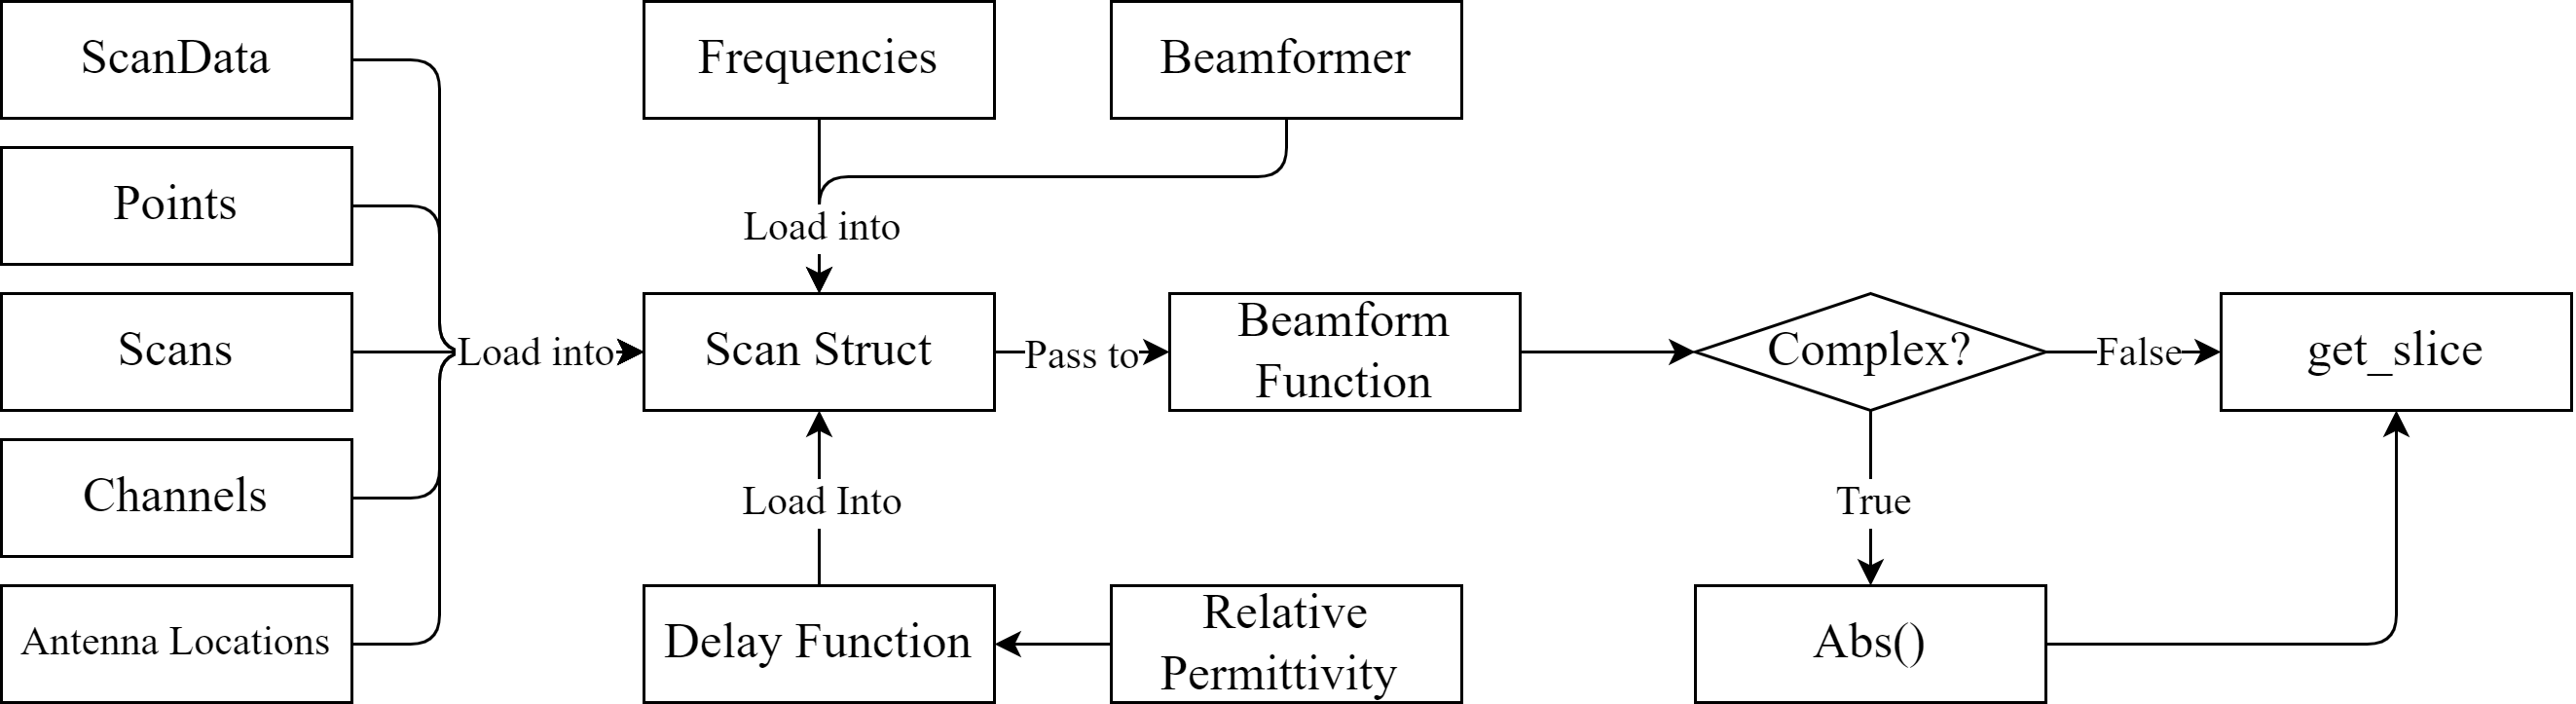
\includegraphics[width=1\textwidth]{MERITWorkflow.png}
    \centering
    \caption{An overview of the current workflow used to image a scan in MERIT.jl} 
    \label{fig:MERITWorkflow}
\end{figure}

This workflow exemplifies how easy it is to use the MERIT.jl library. The function names were deliberately chosen to be
verbose and conform to established nomenclature in the field so that anyone who wants to use the library can understand
what each function does without having to delve into the source code. In this way, the MERIT.jl library is somewhat self
documenting. Additional information is provided above each function in the form of docstrings which can be used with the
help function built into the Julia REPL. 

\section{Plotted Scans}
\label{PlottedScans}
The library was benchmarked against the MATLAB implementation created by Dr. O'Loughlin \textit{et al.} to ensure that
the results provided by MERIT.jl are provably correct. Both implementations were given the same data, B0\_P3\_p000.csv
and B0\_P3\_p036.csv. Rotational subtraction was performed on these in both libraries to reduce the presence of skin
reflections in the data. The data was then processed according to the processing pipeline recommended by both libraries,
the result of which can be seen below in Figure \ref{fig:OutputResults}. It should be noted that the
\lstinline[language=Octave]{imshow} function was used in MATLAB to plot the image. This had the effect of reflecting the
image across the x-axis and also slightly dilating the image along the x-axis, however, since both image matrices share
the same layout, a numerical comparison between the two matrices was possible. The averaged MSE was chosen as the
numerical comparator due to the error squared term in the equation. This causes any small difference to be magnified in
the error, which is desirable when the goal is absolute similarity between the MERIT.jl and its MATLAB counterpart.
Computing the averaged MSE between the two images yielded an error of $8.4417 \times 10^{-7}$ which is within the
accuracy of a float, making it effectively identical to the images produced by MATLAB. This shows that the Julia library
in its current state provides a viable alternative to the MATLAB implementation for frequency domain analysis.

\begin{figure}[t]
    \begin{tabular}{cc}
        \subfloat[MERIT.jl Output]{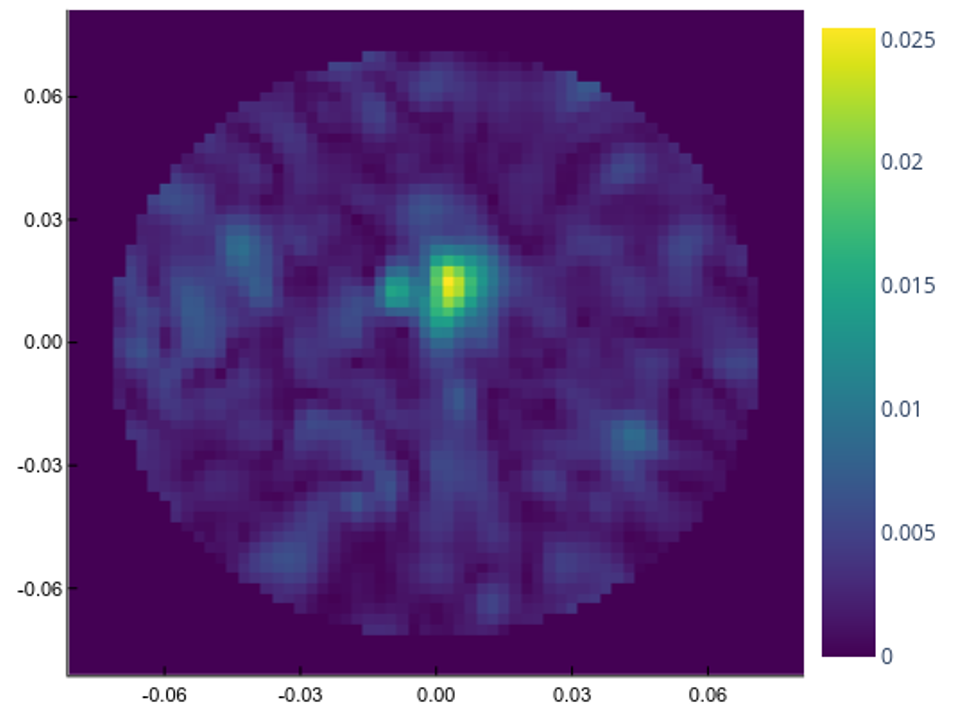
\includegraphics[width=0.45\linewidth]{JuliaOutput.png}}&
        \subfloat[MATLAB Output]{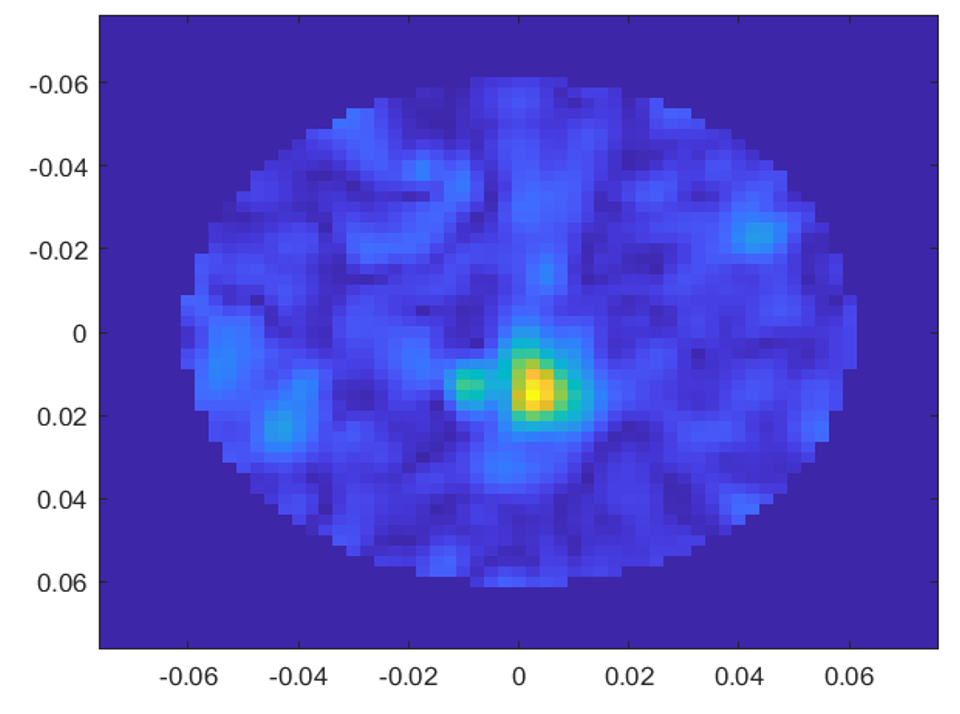
\includegraphics[width=0.45\linewidth]{MATLABOutput.png}}
    \end{tabular}
    \caption{A comparison between Julia and MATLAB output. Averaged MSE of $8.4417 \times 10^{-7}$}
    \label{fig:OutputResults}
\end{figure}

\section{Performance of MERIT.jl}
One of the requirements for MERIT.jl was performance. Through the use of type stability, SIMD optimized for-loops and
the disabling of array bounds checking, the library could process the provided data in 8 seconds. However, after the
addition of the Points data type for type safety, the processing time climbed to 12 seconds. While the overall runtime
is still acceptable, an increase of 3 seconds is less than ideal. An analysis to narrow down the cause of the increased
runtime could not be conducted, however, unoptimized functions from the Points library may be the culprit. To capture
the full performance characteristics of the library, a scalability test was performed, in which the number of points,
channels and frequency divisions were progressively increased. This was performed in an automated manner using the
functions provided by BenchmarkTools.jl \cite{BenchmarkToolsJl}. The results from the benchmark suites were
exported to CSV files and analyzed in Excel to judge the ``Big O'' notation of MERIT.jl.

\begin{figure}[h!]
    \begin{tabular}{cc}
        \subfloat[Raw Points]{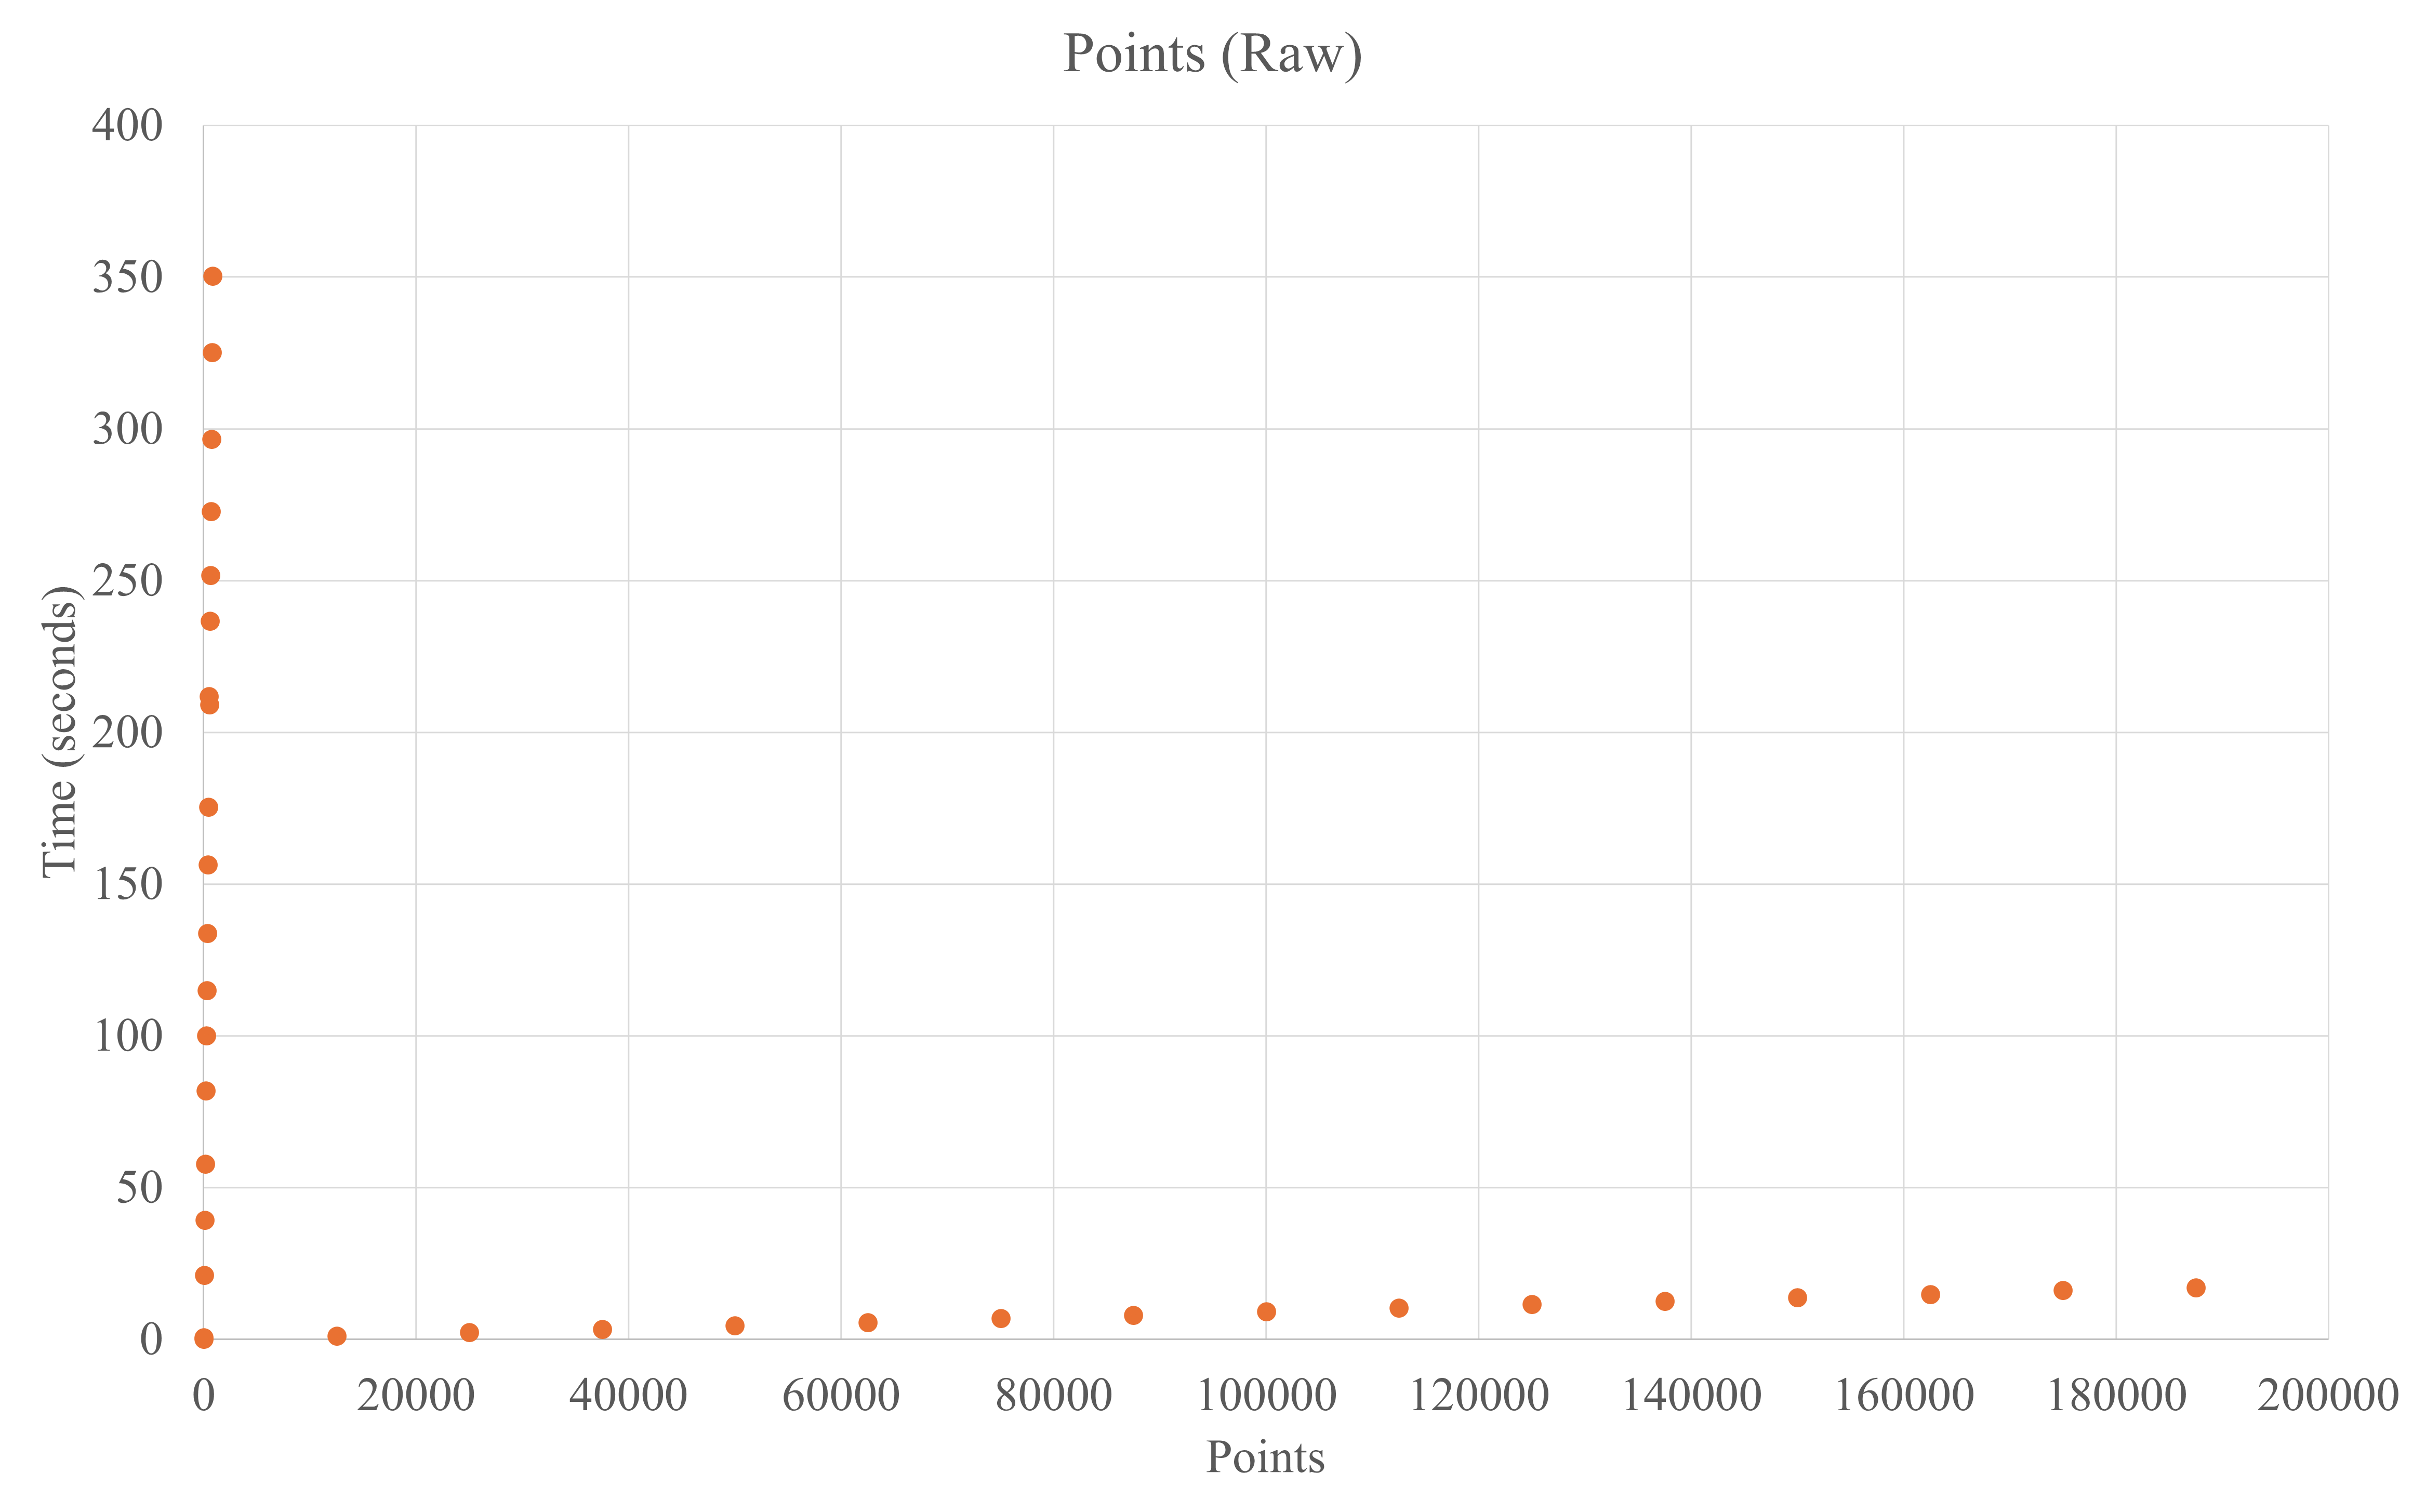
\includegraphics[width=0.45\linewidth]{PointsUnedited.png}}&
        \subfloat[Processed Points]{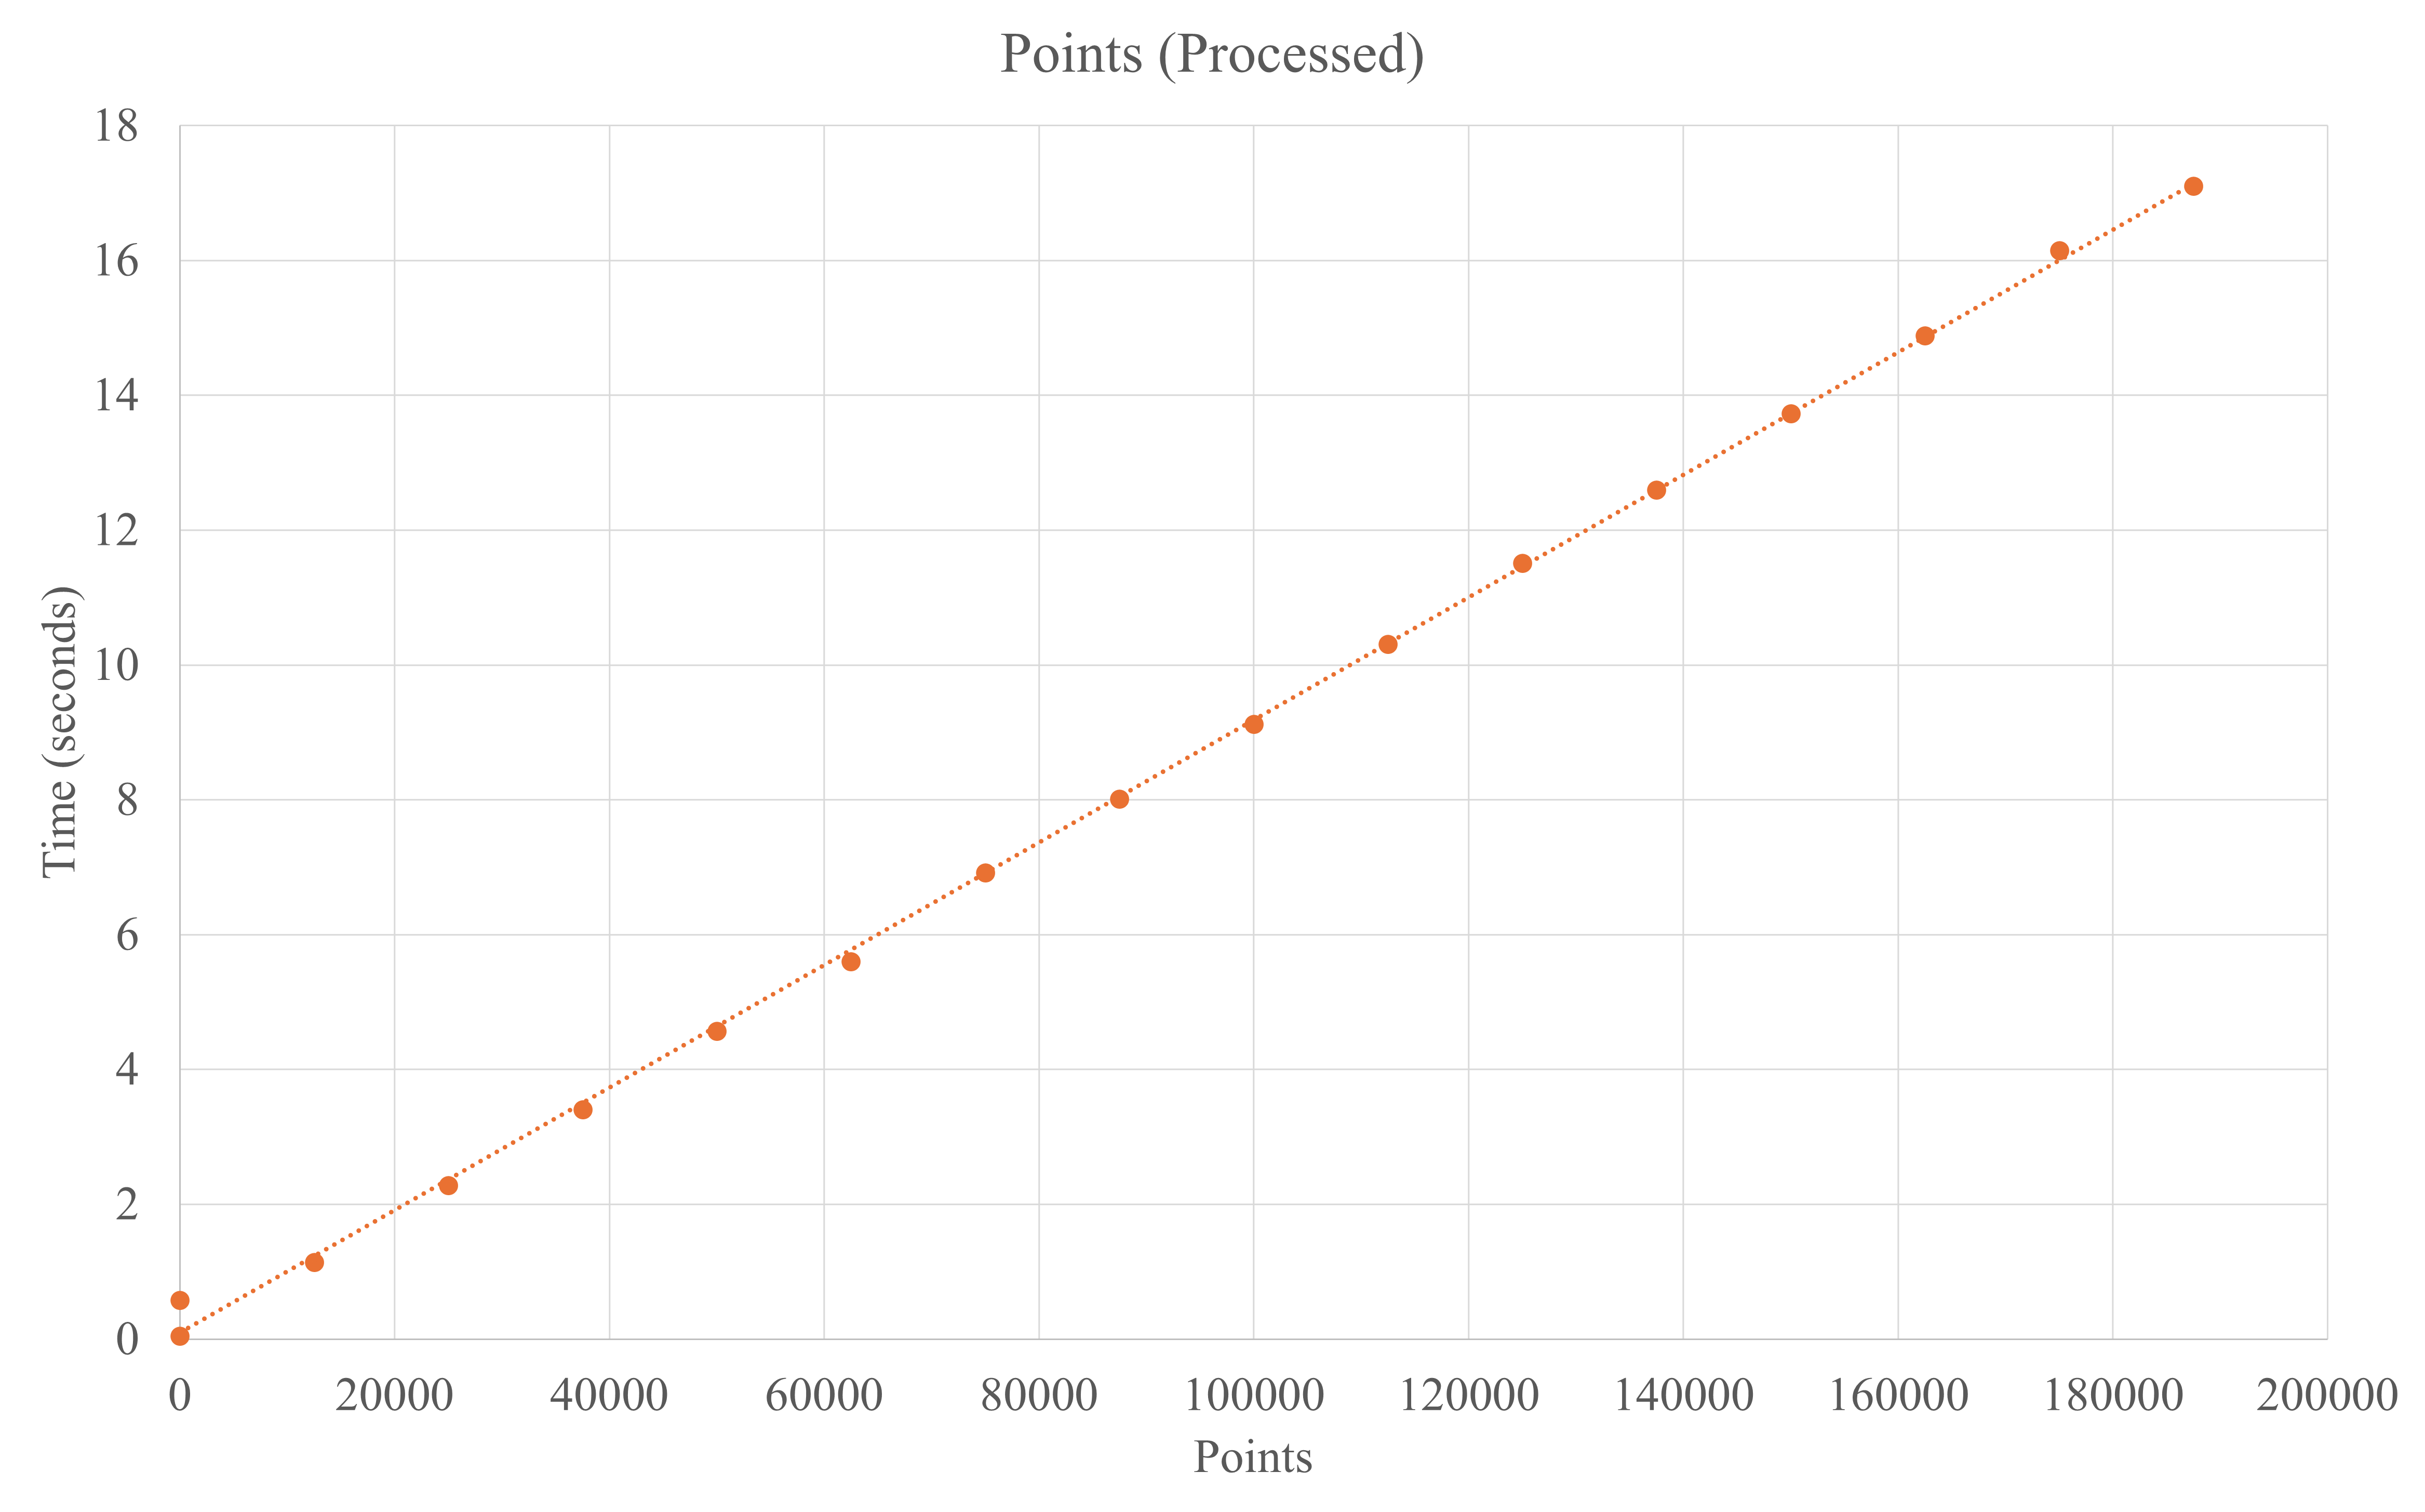
\includegraphics[width=0.45\linewidth]{PointsEdited.png}}
    \end{tabular}
    \caption{Runtime for increasing Points}
    \label{fig:PointsResults}
\end{figure}

\begin{figure}[h!]
    \centering
    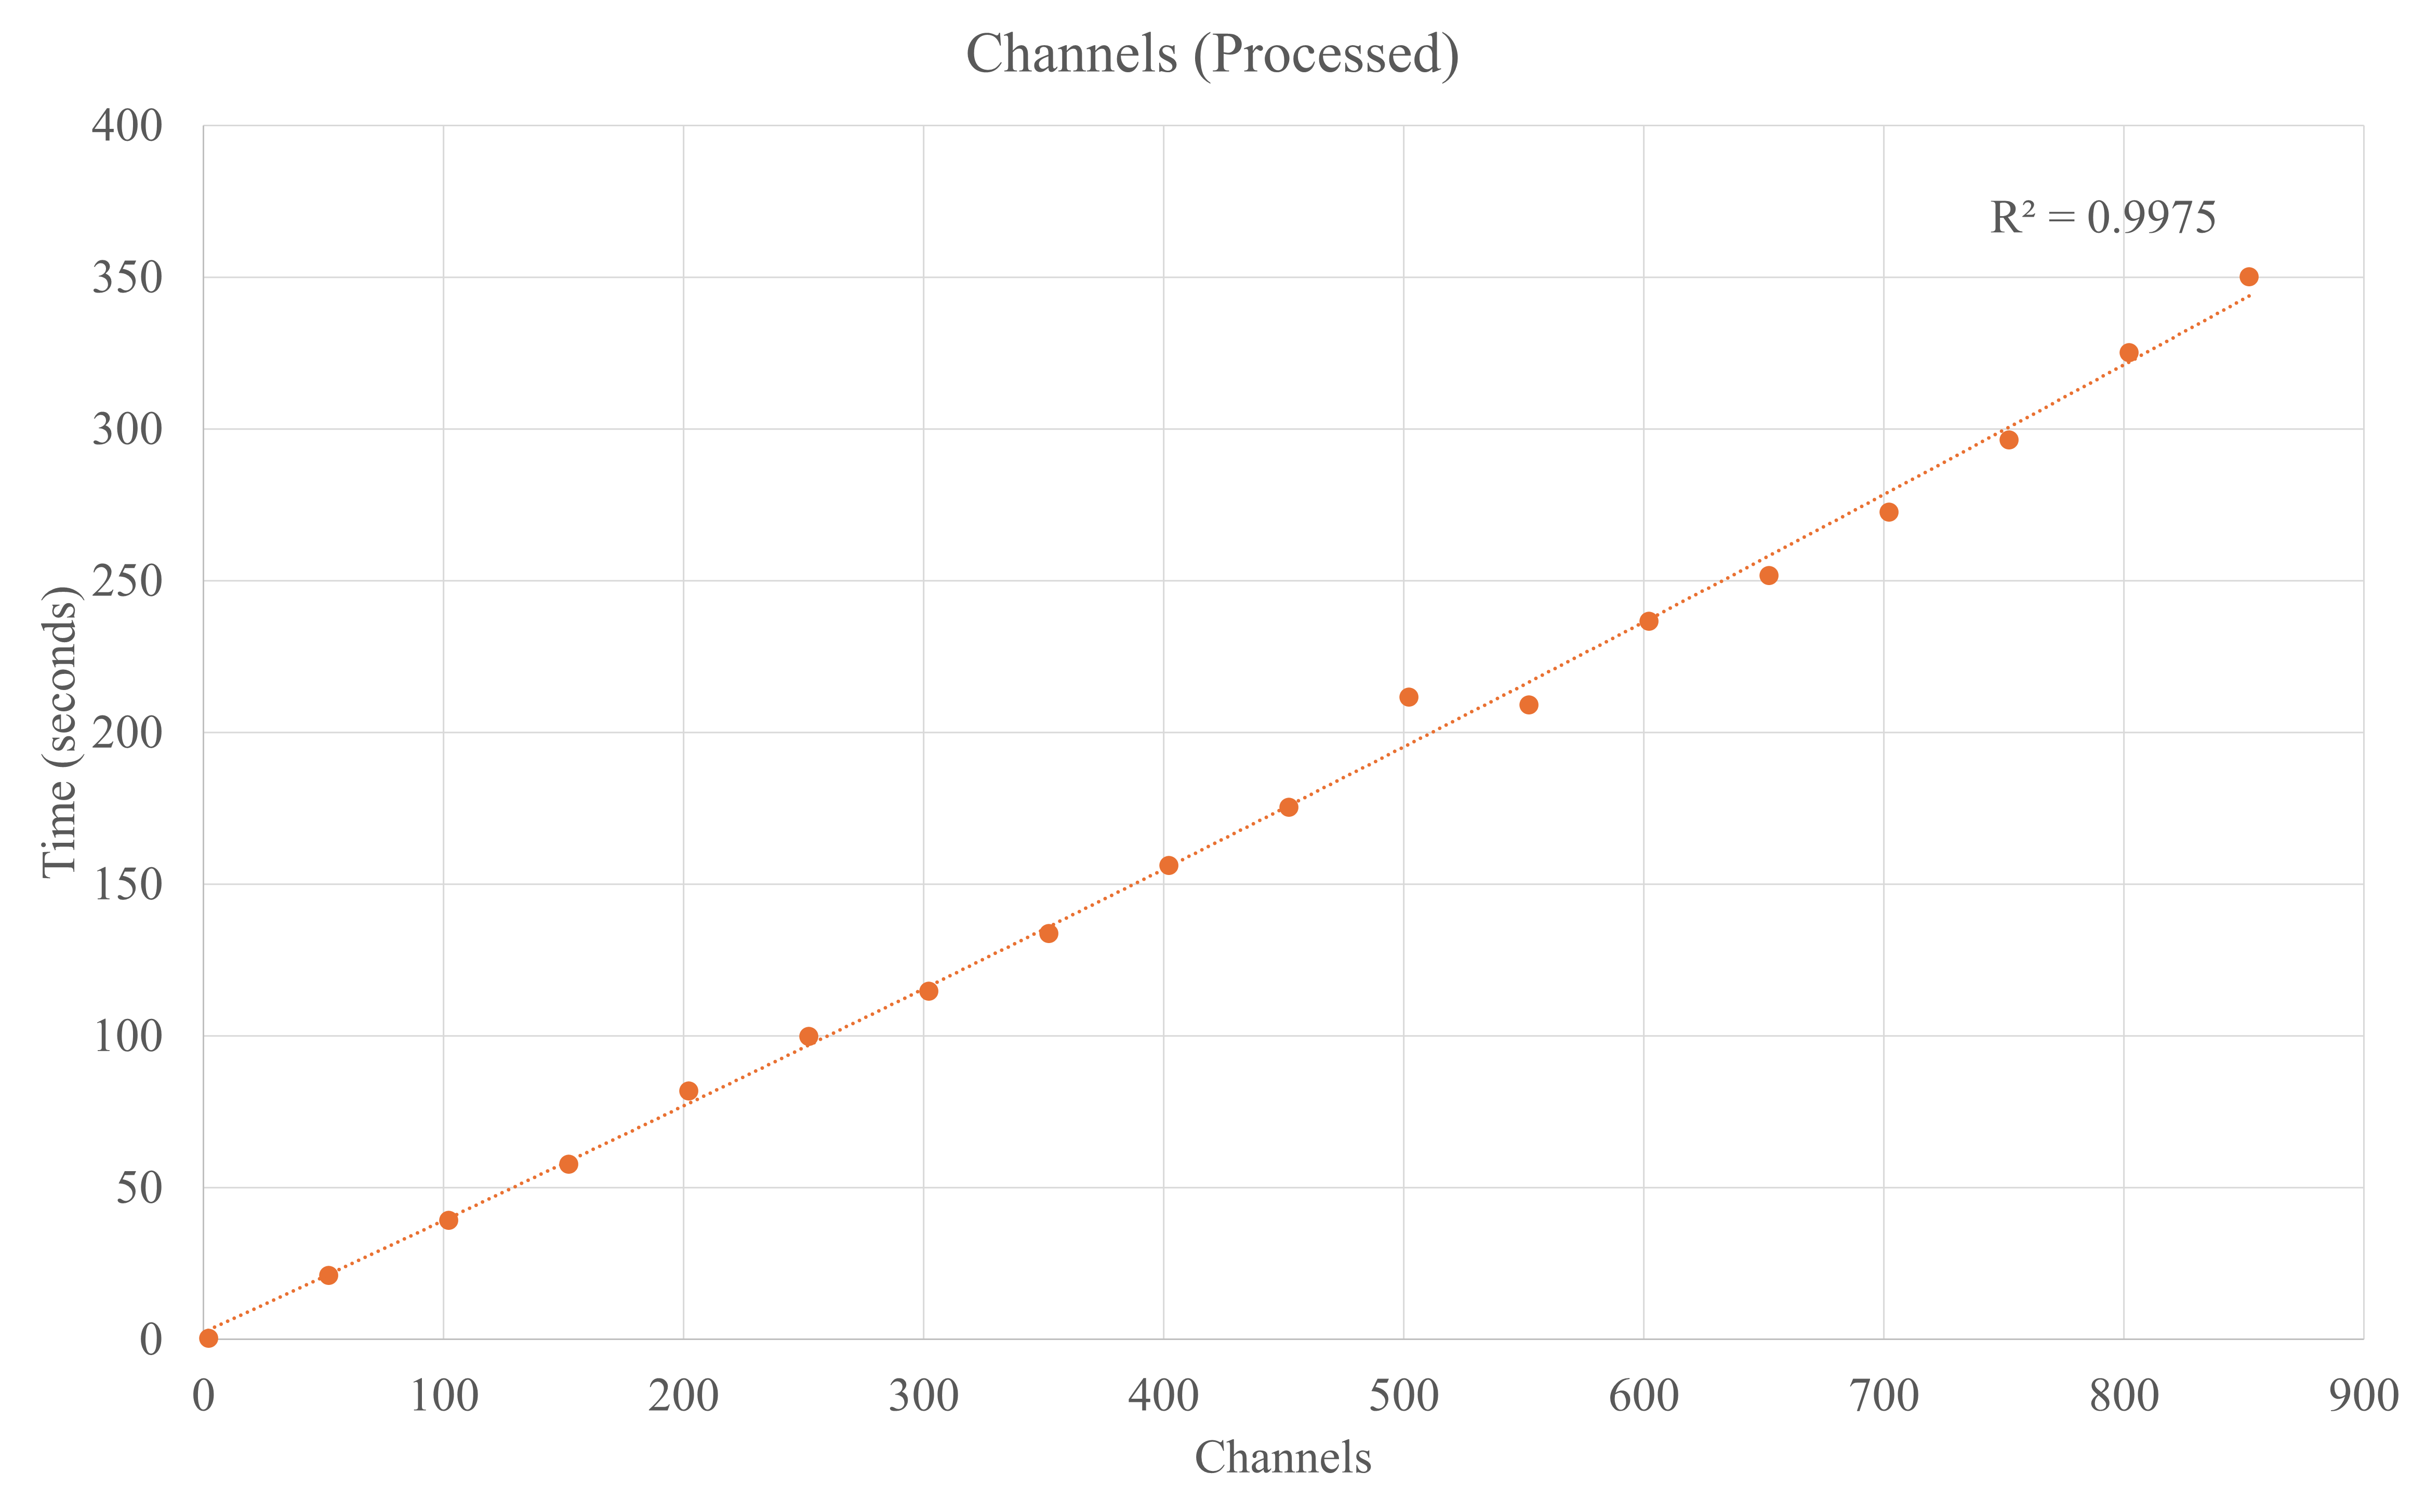
\includegraphics[width=0.75\linewidth]{ChannelsUnedited.png}
    \caption{Runtime for increasing Channels}
    \label{fig:ChannelsResults}
\end{figure}
\vspace{1mm}
\begin{figure}[h!]
    \begin{tabular}{cc}
        \subfloat[Raw Frequencies]{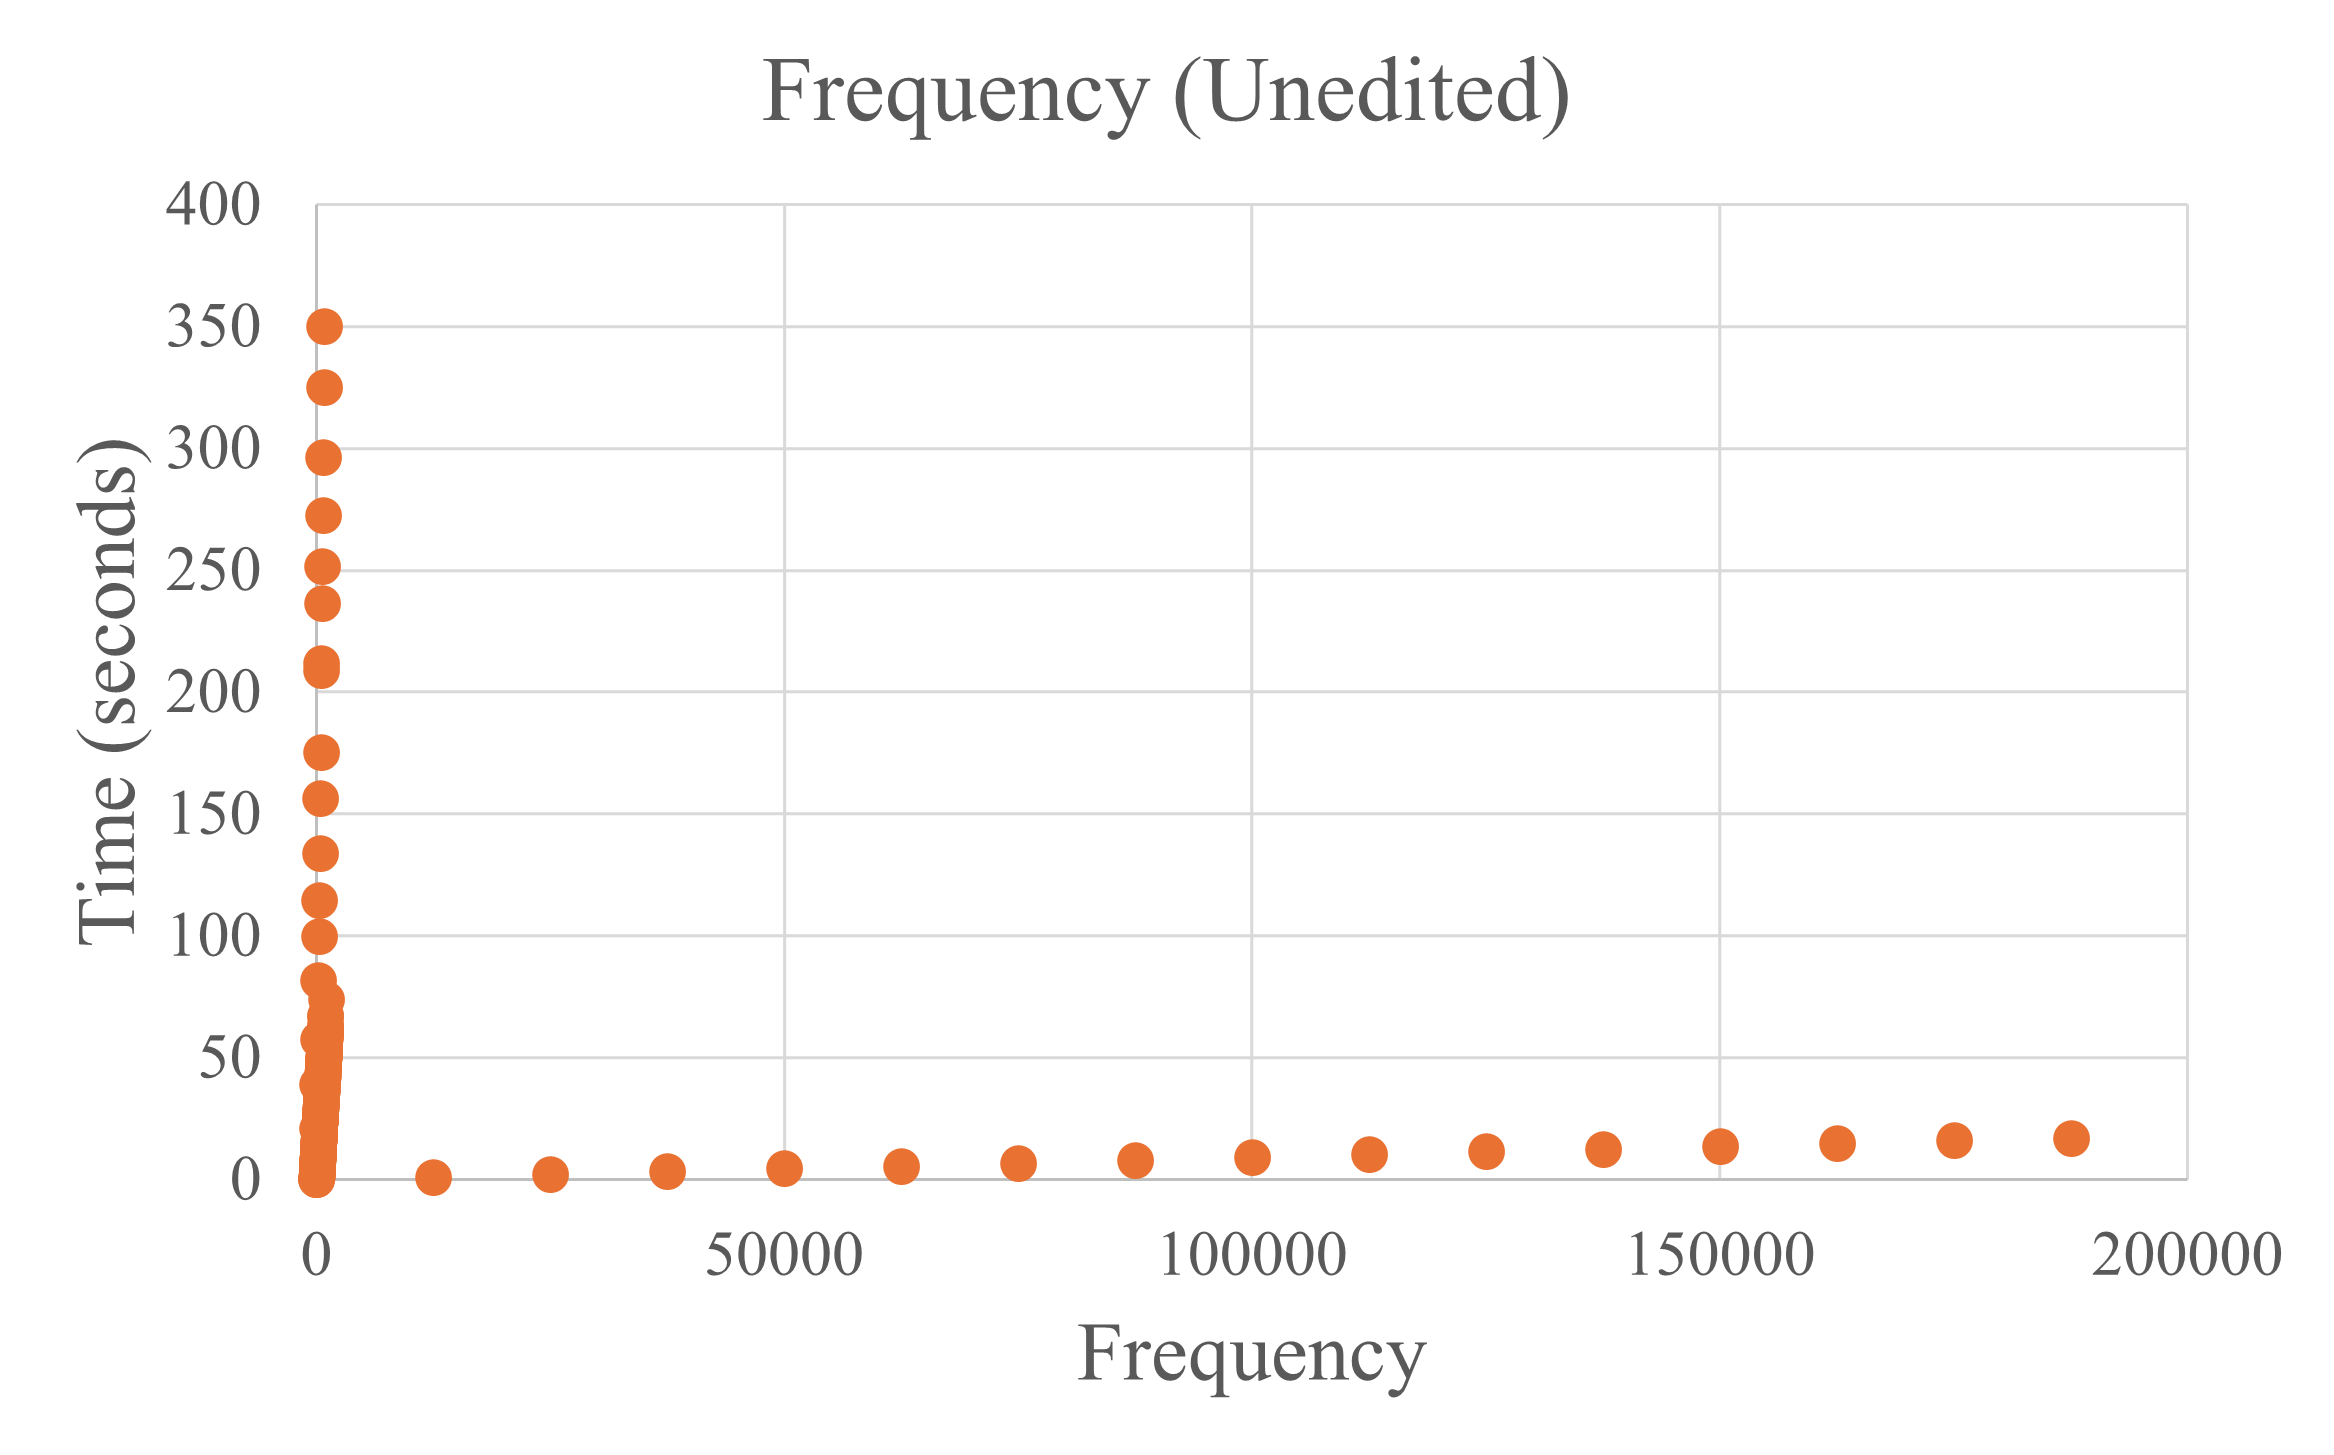
\includegraphics[width=0.45\linewidth]{FrequencyUnedited.png}}&
        \subfloat[Processed Frequencies]{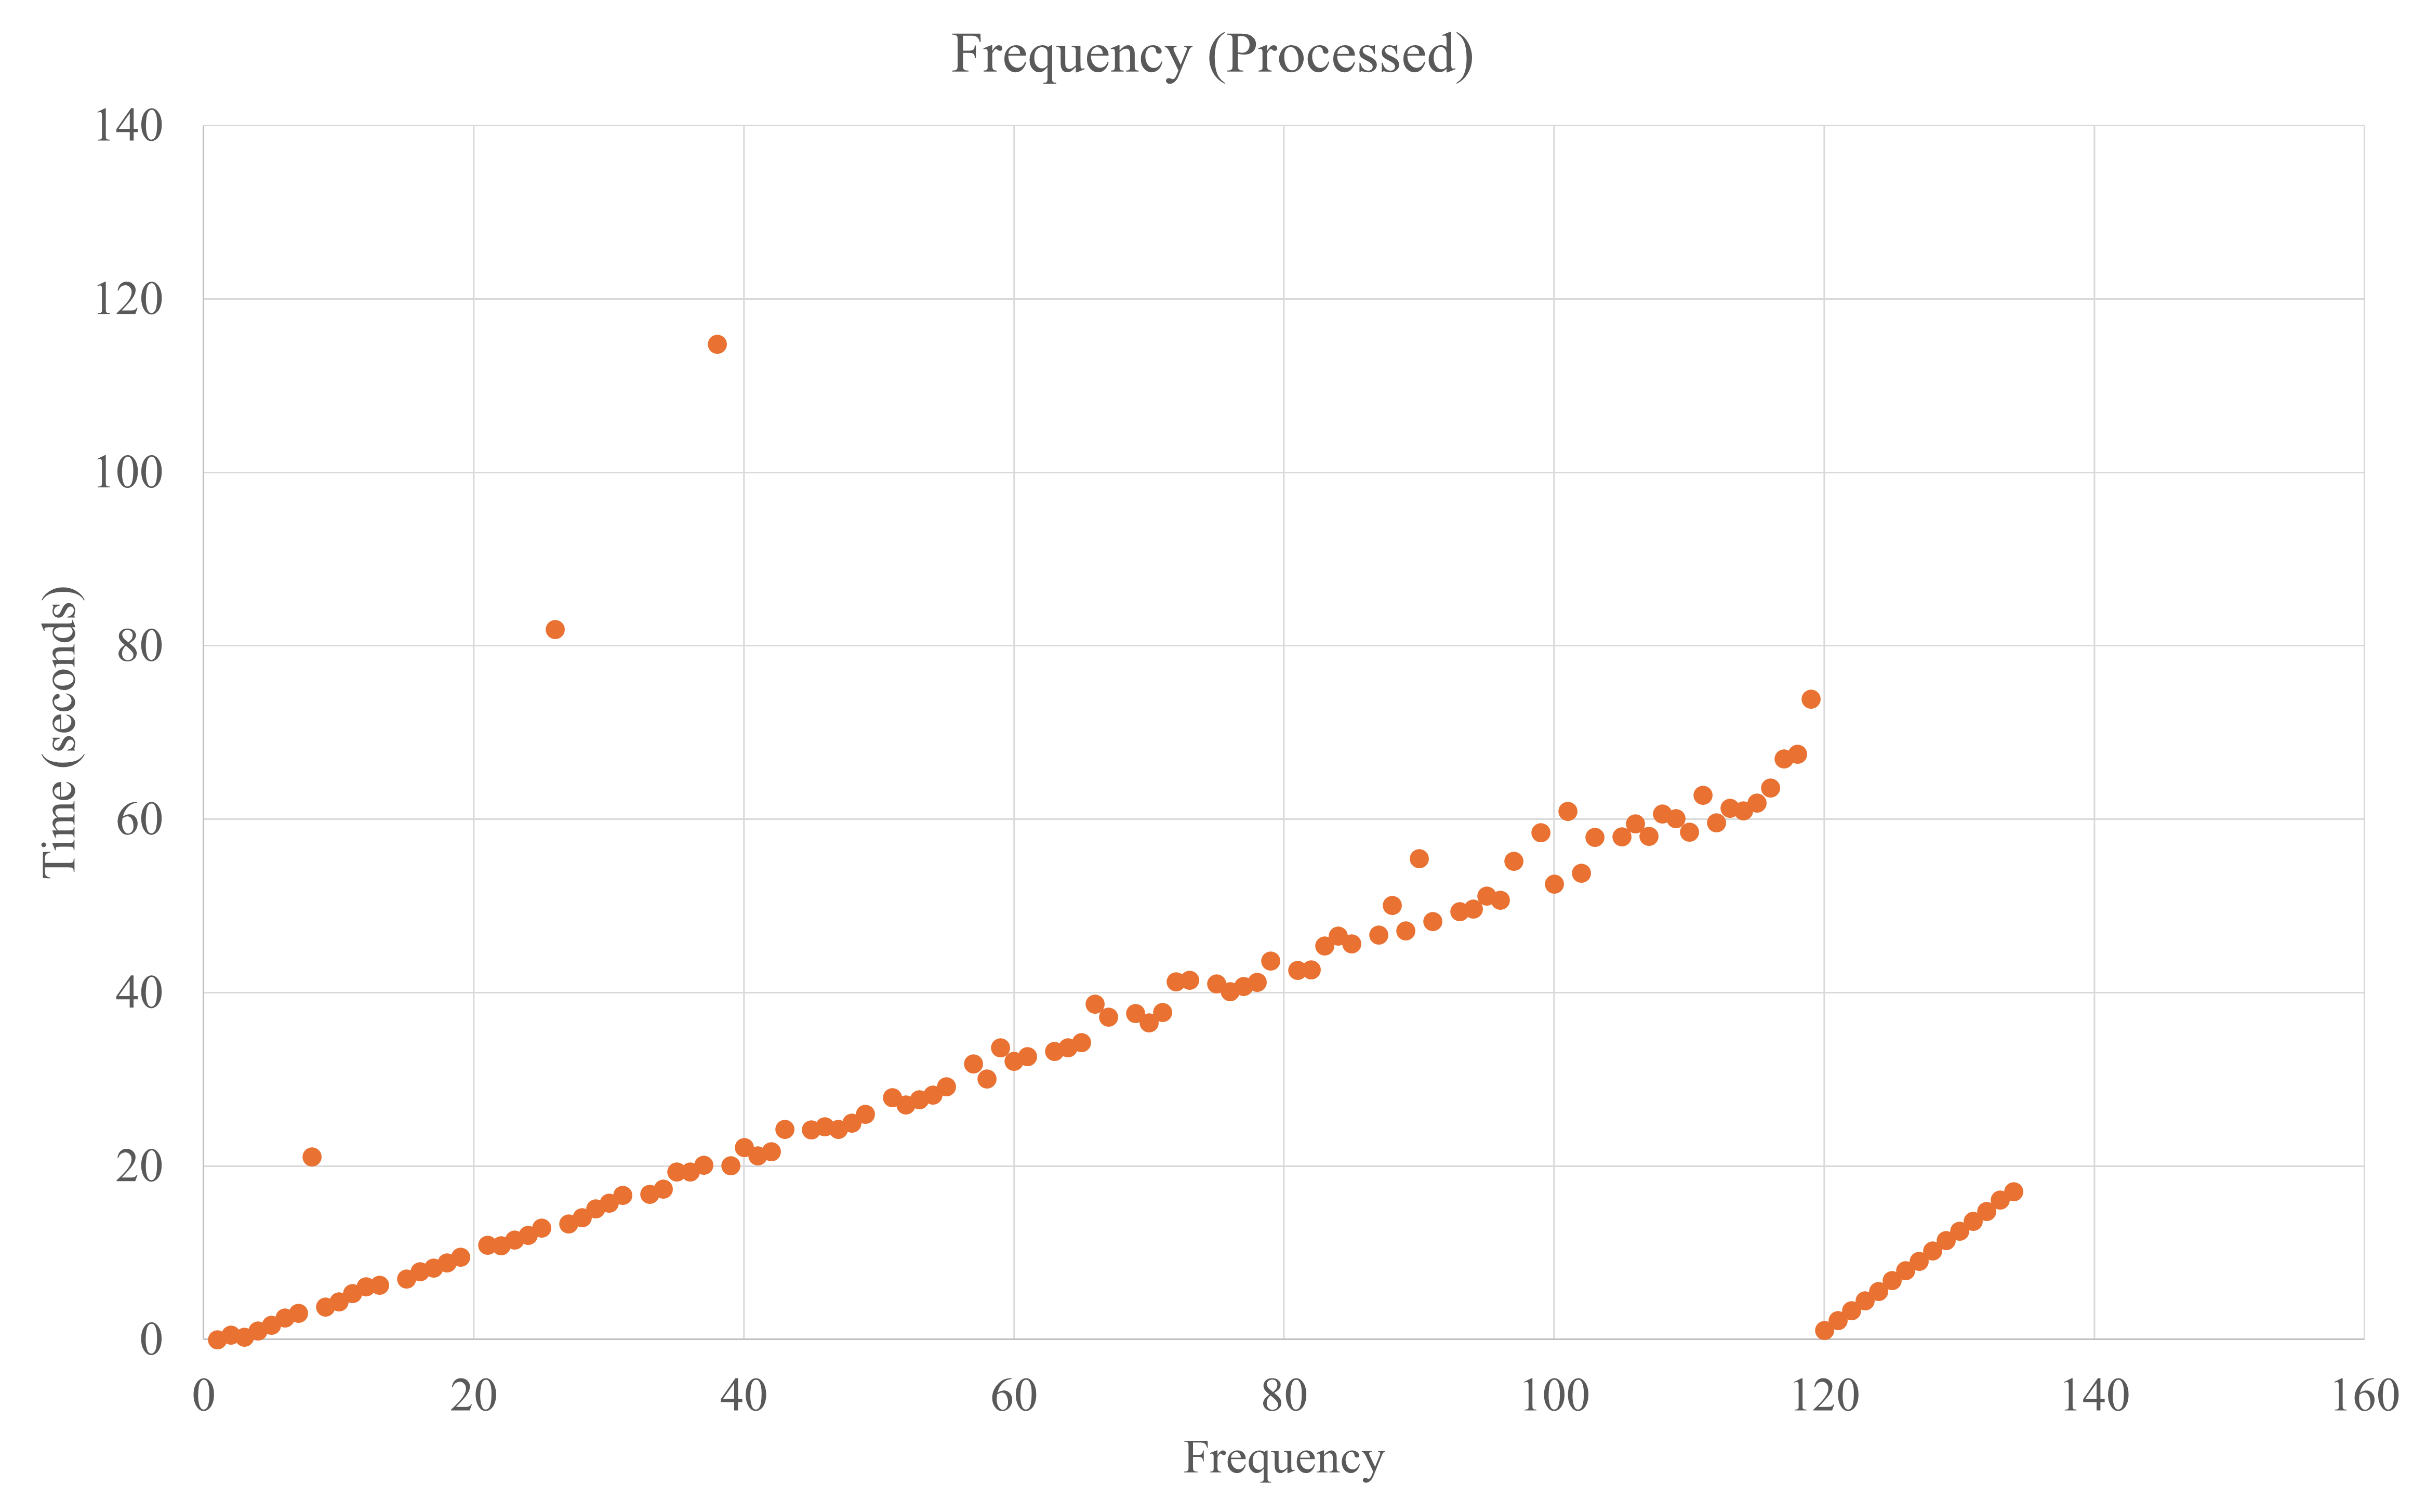
\includegraphics[width=0.45\linewidth]{FrequencyEdited.png}}
    \end{tabular}
    \caption{Runtime for increasing Frequency divisions}
    \label{fig:FrequenciesResults}
\end{figure}

Figures \ref{fig:PointsResults}, \ref{fig:ChannelsResults}, \ref{fig:FrequenciesResults} show the results from
BenchmarkTools. A large number of outliers were found, as can be seen in the raw data charts. Subsequent analysis
revealed that these outliers were the product of excessive usage of the swap file on the test system; a consequence of
the insufficient amounts of available RAM and the large overhead introduced by the BenchmarkTools library. Since these
data points are an artifact caused by the BenchmarkTools library, they were removed from the data set. A curve was
fitted to the remaining points, to indicate the time complexity. From this analysis, it was concluded that MERIT.jl
scales linearly with the number of points ($\mathcal{O}(n)$) as can be seen in Figure \ref{fig:PointsResults}, and
quadratically with the number of channels ($\mathcal{O}(n^2)$) as seen by the slightly quadratic increase in Figure
\ref{fig:ChannelsResults}. This aligns with expectations based on an algorithm analysis of the DAS beamformer. The main
loop consists of a single for loop iterating over the points as such, the algorithm is expected to behave linearly with
an increase in points. With channels, every additional antenna corresponds to a quadratic increase in channels since
every antenna can send to and receive from any other antenna in a fully multistatic system. The algorithm is expected to
have $\mathcal{O}(n)$ growth in the number of frequency divisions since they are only used once in the algorithm process
to delay each signal. This is evidenced by the linear growth trend that can be seen in Figure
\ref{fig:FrequenciesResults}. Effectively, MERIT works very well with a large number of points and with relatively few
channels. This in turn affected the layout of the matrices in the library. Since data to do with points would be
accessed most frequently, it was decided to place this data along the columns of the matrices. Since Julia is a column
major language, this would provide the quickest access to this data. Data that relate to the channels were placed along
the second dimension since this would be accessed less frequently than data related to the points. Finally, data
relating to the frequency were placed along the third dimension, since this data is accessed very infrequently, it was
decided that the latency required to load this data from memory would be acceptable provided it allowed us easy access
to data relating to points and channels. The above graphs demonstrate the performance of the MERIT.jl library. From
limited testing on my laptop with an Intel i7-1185G7 CPU, the Julia library executed in the same amount of time as its
MATLAB counterpart. However, further testing to accurately quantify the runtime of both libraries is needed.

\section{MERIT.jl as a Library}
\label{MERITAsLibrary}
Creating generalized software for research is a challenge as most researchers create software and libraries that are
specific to the question they are trying to answer. Conducting a search for microwave imaging libraries on Github yields
23 repositories coded in either MATLAB, Python, C, C++ or R which upon further inspection were all created to solve a
particular research question. For example, DLMiMed was created to investigate the use of deep learning for breast tumor
classification in medical microwave images \cite{gerazovDLMiMed17}. Other researchers who might want to answer other
questions relating to deep learning in microwave imaging cannot make use of this repository due to its fixed neural
network and lack of generalizable code. Another example is the ``Microwave-Imaging'' repository created by André and
Lucas Batista and Ricardo Adriano for their implementation of a quadratic programming approach to microwave breast
imaging \cite{batistaMicrowaveImaging21}. Again, this repository is specific to their research question and is only
useful to researchers who want to investigate similar questions. Also, it is not clear how one could extend this
repository to answer other questions in the field of microwave imaging in a way that is transparent to the end user.
Only the MERIT library created by Dr. O'Loughlin stood out as a truly generalized library by providing researchers with
3 well known beamforming algorithms, as well as helper functions that would allow them to visualize the provided scan
data. This is the gap that MERIT.jl aims to fill. Section \ref{CurrentWorkflow} shows how quick and easy it would be for
a researcher to ingest their data into the BreastScan struct and to visualize the output. Through the use of closure as
mentioned in section \ref{ClosureMJL}, MERIT.jl allows for extensive flexibility for the choice of $\varepsilon$, which
is a parameter that is often changed by researchers. MERIT.jl also provides researchers with flexibility in the choice
of delay and beamforming function used. 
\begin{lstlisting}[language=Julia]
function delay_template(relative_permiativity)
    # Capture the relatively_permiativity
    
    # Create a delay function
    function calc_(channels, antenna, domain_points):
        #calculate and return a time matrix
        #Size = (1 x #Channels x #Points)
    end
end

function beamformer(delayed_signals)
    #Do some processing
    #return should be of size (1 x 1 x #Points)
end
\end{lstlisting}
By creating a delay and beamformer function that follows the template provided above, researchers can substitute their
own functions into the BreastScan struct and the one-call processing pipeline will work as normal. Section
\ref{JuliaScientificComputing} showcased how easy it was for the DifferentialEquations.jl module to extend the classes
and functions already provided in SciMLBase so that structures from one library could be used with functions from another
library in a way that was completely transparent to the end users, by leveraging the aforementioned features in Julia.
Since MERIT.jl also makes use of these features, it also benefits from the easy extensibility that comes as a
consequence.